\documentclass[hidelinks,a4paper,14pt]{article}
\usepackage{ amsmath, amssymb}
\usepackage{graphicx}
\usepackage{color,amsmath,graphics,graphicx}
\usepackage{amsfonts}
\usepackage{mathrsfs,hyperref}
\usepackage{latexsym,amsmath,enumerate,amsbsy,amsthm}
\textwidth = 415pt

%==============================================
\usepackage{fontspec}
\usepackage{xunicode}
\usepackage{xltxtra}
\defaultfontfeatures{Scale=1.23}
\XeTeXlinebreaklocale “th_TH” % สำหรับตัดคำ
\setmainfont[Scale=1.23]{TH SarabunPSK}
%==============================================
%%%%%%%%%%%%%%% THEOREM Environments %%%%%%%%%% 
\newtheorem{theorem}{ทฤษฎีบท}[section]						%
\newtheorem{lemma}[theorem]{บทตั้ง}						%
\newtheorem{conjecture}[theorem]{บทคาดการณ์}				%
\newtheorem{definition}[theorem]{บทนิยาม}					%
\newtheorem{remark}[theorem]{หมายเหตุ}						%
\newtheorem{proposition}[theorem]{ประพจน์}					%
\newtheorem{corollary}[theorem]{บทแทรก}					%
\numberwithin{equation}{section}							%
\newtheorem{example}[theorem]{ตัวอย่าง}						%
%\newtheorem{exercise}{แบบฝึกหัด}[chapter]	
%\renewcommand{\chaptername}{บทที่}
\renewcommand\tablename{ตารางที่}
\renewcommand\figurename{รูปที่}
\renewcommand{\contentsname}{สารบัญ}						%
%\renewcommand{\bibname}{บรรณานุกรม}						% 
\renewcommand{\indexname}{ดรรชนี}					%
%%%%%%%%%%%%%%%%%%%%%%%%%%%%%%%%%%%%%%%%%%%%%%%
% addition mod
\usepackage{subcaption,float,framed,algorithm2e,hyperref}
%%%%


\begin{document}
	{\begin{center}
			\textbf{Project Proposal}\\
			\vspace{0.5cm}
			\textbf{Division of Applied Mathematics, Department of Mathematics}\\
			\vspace{0.5cm}
			\textbf{Faculty of Science, Silpakorn University}
		\end{center}}
		{
			\vspace{0.5cm}
			\flushleft{Date : { 27 กันยายน 2561 } \hfill{ }}
			\flushleft{Advisor : {  ผู้ช่วยศาสตราจารย์ ดร. นพดล  ชุมชอบ}}\\
			\flushleft{Student : { นายภัคพล       พงษ์ทวี     รหัส  07580028}\\
			\vspace{1cm}
		}
		
		
		% Here the project title
		{\textbf{\begin{flushleft}Project Title : ลบบทบรรยายแบบแข็งบนวิดีโอแบบอนิเมะ \\
				(Hard-coded subtitle remover for anime)
			\end{flushleft}
		}}
		\thispagestyle{empty}
	\section{Introduction}
	\setlength\parindent{24pt}\hspace{\parindent} %addition mod: Tab
	 บทบรรยายใต้ภาพ (subtitle) คือข้อความที่ได้จากการถอดเสียงจาก ภาพยนตร์ รายการทีวี หรือสื่อต่างๆ ที่มักแสดงอยู่ที่ด้านล่างของหน้าจอ ซึ่งใช้เพื่อแสดงคำแปลในภาษาอื่น หรือเพื่อช่วยเหลือผู้ประสบปัญหาทางการได้ยิน โดยบทบรรยายใต้ภาพ แบ่งตามการสร้างได้เป็น 2 ประเภทได้แก่ แบบ Soft และแบบ Hard โดยแบบ Soft จะมีลักษณะเป็นข้อความที่ถูกระบุตำแหน่งเวลาไว้ สามารถเปิดและปิดได้ แต่ก็มีปัญหาว่าเครื่องเล่นหรือซอร์ฟแวร์ที่ใช้จำเป็นต้องรองรับรูปแบบบทบรรยายนั้นจึงจะแสดงขึ้นมาได้ และในบางครั้งก็มีปัญหาด้านการเข้ารหัส ทำให้ไม่สามารถแสดงข้อความได้อย่างถูกต้องและแบบ Hard คือ ข้อความในบทบรรยายจะถูกฝังรวมเป็นเนื้อเดียวกับวิดีโอ ซึึงวิธีนี้จะทำให้ไม่จำเป็นต้องใช้เครื่องเล่นหรือซอร์ฟแวร์พิเศษเพื่อรองรับ ทำให้ไม่มีปัญหาในการแสดงผล แต่ว่าบทบรรยายแบบนี้จะไม่สามารถทำการเปิดและปิดได้\newline 
	
	จากการที่บทบรรยายใต้ภาพแบบ Hard ไม่สามารถเปิดและปิดได้ทำให้บทบรรยายดังกล่าวก่อกวนผู้รับชม ตัวอย่างเช่น ภาพยนตร์จีนกำลังภายในที่ฉายทางโทรทัศน์ไทยมักจะมีบทบรรยายภาษาจีนติดมาด้วย เนื่องจากประเทศจีนมีการใช้ภาษาจีนในสำเนียงที่หลากหลาย จึงมีบทบรรยายให้สามารถรับชมได้โดยเข้าใจความหมายที่เหมือนกัน โดยคำบทบรรยายที่ใช้นั้น เป็นบทบรรยายแบบ Hard ซึ่งเมื่อภาพยนตร์ดังกล่าวได้รับการให้เสียงไทยแล้ว ภาพยนตร์จึงมีบทบรรยายภาษาจีนติดมาด้วย \newline
	
	ด้วยปัญหาที่กล่าวมาข้างต้นโดยผู้ศึกษาได้มีความสนใจที่จะลบบทบรรยายแบบ Hard ออกจากวิดีโอ โดยเฉพาะวิดิโอแบบอนิเมะ เนื่องจากวิดีโอประเภทนี้มักมีบทบรรยายติดมาด้วย และบางครั้งมีบทบรรยายเป็นแบบ Hard ทำให้ไม่สามารถเปิดและปิดได้ ซึ่งการลบบทบรรยายนี้ ซึ่งการลบบทบรรยายออกจากวิดีโออนิเมะ เปรียบได้กับการซ่อมภาพศิลปะที่เสียหาย ในอนาคตสามารถพัฒนาต่อยอดได้เป็นแอปพลิเคชันที่จะสามารถนำโทรศัพท์มือถือส่องไปยังงานศิลปะที่เสียหายและทำการซ่อมแซมภาพนั้นและแสดงขึ้นบนหน้าจอแบบเรียลไทม์ได้\newline
	
	โดยวิดีโอนั้นประกอบด้วยภาพจำนวนหลายภาพต่อหนึ่งหน่วยเวลา เราจะเรียกภาพหนึ่งภาพในวิดีโอว่า เฟรม (frame) ซึ่งภาพในแต่ละเฟรมเรียกว่าภาพดิจิตัล (Digital Image) โดยภาพดิจิตัลนั้นจะสามารถนิยามได้เป็นฟังก์ชัน $f(x,y)$ โดยที่ $x$ และ $y$ เป็นพิกัดของภาพ และแอมพิจูดของ $f$ ที่พิกัด $(x,y)$ ใดๆ ในภาพคือค่าความเข้มแสง (intensity)  ซึ่งแอมพิจูดนี้มีค่าจำกัด\newline
	
	ซึ่งก่อนจะลบบทบรรยายนั้น จะเป็นต้องหาบทบรรยายในภาพให้ได้เสียก่อน โดยบทบรรยายของอนิเมะนั้น มักจะขึ้นบริเวณด้านล่างของหน้าจอ และนอกจากนี้ บทบรรยายอนิเมะมักจะใช้ขอบของตัวอักษรเป็นสีดำอีกด้วย ด้วยสมบัตินี้เองทำให้เราสามารถหาบริเวณบนเฟรมที่เป็นบทบรรยายได้โดยจะมีวิธีหาพื้นที่ซึ่งเป็นบทบรรยายดังนี้
	
	\begin{figure}[H]
		\begin{subfigure}{0.4\linewidth}
			\centering
			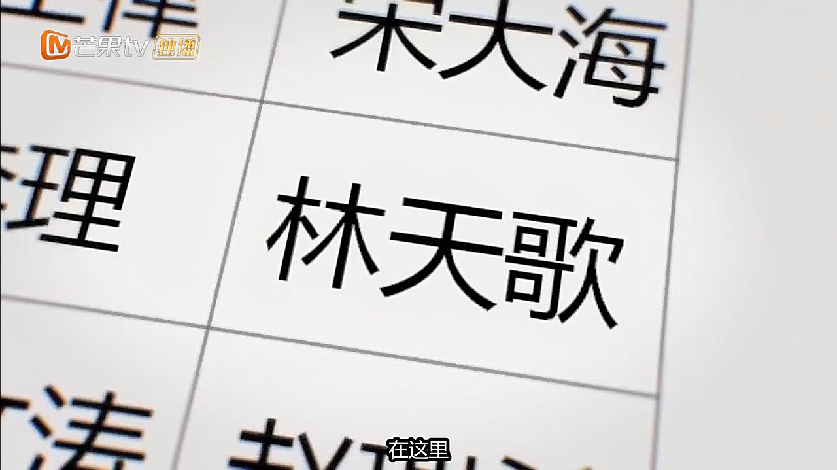
\includegraphics[width=0.4\linewidth]{images/detection-original.png}
			\caption{ภาพเฟรมอนิเมะที่มีบทบรรยาย}
		\end{subfigure}
		\begin{subfigure}{0.4\linewidth}
			\centering
			
\includegraphics[width=0.4\linewidth]{images/detection-threshold.png}
			\caption{ภาพหลังทำการตัดส่วนล่างและ thresholding}
		\end{subfigure}
	\end{figure}
	
ตัดเฟรมมาเฉพาะส่วนล่างของเฟรมที่น่าจะมีบทบรรยายปรากฏอยู่ จากนั้นทำการ thresholding เพื่อหาบริเวณที่เป็นสีดำเนื่องจากบทบรรยายจะถูกล้อมรอบด้วยสีดำเสมอ

\begin{figure}[H]
	\begin{subfigure}{0.4\linewidth}
		\centering
		
\includegraphics[width=0.4\linewidth]{images/detection-inverse.png}
		\caption{ภาพหลังทำการสลับสีี}
	\end{subfigure}
	\begin{subfigure}{0.4\linewidth}
		\centering
		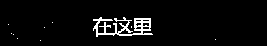
\includegraphics[width=0.4\linewidth]{images/detection-blackfill.png}
		\caption{ภาพหลังทำการเปลี่ยนพื้นที่สีขาว}
	\end{subfigure}
\end{figure}

ทำการสลับสีระหว่างสีดำกับสีขาวของภาพที่ทำการ thresholding หลังจากนั้นทำการเปลี่ยนพื้นที่สีขาวซึ่งติดกับขอบของเฟรมทั้งหมดให้เป็นสีดำ เพราะว่า บทบรรยายไม่อยู่ติดกับหน้าจอ เราจะถือว่าสิ่งที่อยู่ติดกับหน้าจอไม่ใช่บทบรรยาย

\begin{figure}[H]
	\begin{subfigure}{0.4\linewidth}
		\centering
		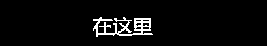
\includegraphics[width=0.4\linewidth]{images/detection-erode-opening.png}
		\caption{ภาพหลังการ erode และ opening}
	\end{subfigure}
	\begin{subfigure}{0.4\linewidth}
		\centering
		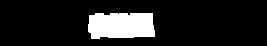
\includegraphics[width=0.4\linewidth]{images/detection-stoke.png}
		\caption{ภาพหลังการ dilate}
	\end{subfigure}
\end{figure}

จากนั้นนำวัตถุที่มีขนาดเล็กเกินไป หรือใหญ่เกินไปออกจากภาพด้วยวิธีการ erode และ opening
จะได้ว่าส่วนที่เหลือเป็นสีขาวในภาพคือบทบรรยาย แต่ว่าขอบของบทบรรยายก็ต้องถูกลบออกไปด้วย จึงทำการ dilate เพื่อขยายขอบของบทบรรยายให้เท่ากับบทบรรยายที่อยู่ในเฟรมวิดีโอ และสิ่งที่เหลืออยู่คือ inpaint domain ที่จะนำไปใช้ในการซ่อมแซมภาพต่อไป
	
	การซ่อมแซมภาพ คือกระบวนการที่จะเติมเต็มข้อมูลที่หายไปในพื้นที่ภาพที่กำหนด โดยมีจุดประสงค์เพื่อซ่อมแซมภาพที่เสียหาย โดยพื้นที่ภาพส่วนนั้นไม่สามารถพบได้จากการสังเกต โดยการกู้คืน สี, โครงสร้าง และพื้นผิว ที่เกิดการเสียหายเป็นวงกว้าง พิกเซลที่จะนำมาใช้ซ่อมแซมจะถูกคำนวณขึ้นมาใหม่จากข้อมูลที่พิกเซลที่อยู่โดยรอบที่ยังไม่เสียหาย \cite{ref:defination-of-inpaint}  ซึ่งการจะนำบทบรรยายออกจากเฟรมวิดีโอนั้น จะพิจารณาว่าบทบรรยายนั้นเป็นส่วนที่เสียหาย แล้วจากนั้นจึงใช้การซ่อมแซมภาพเพื่อนำบทบรรยายนั้นออก\newline
	
	การซ่อมแซมรูปภาพมีวิธีการทางคณิตศาสตร์ที่ใช้แตกต่างกันไปจำนวนมาก แต่การซ่อมแซมด้วยการแปรผันจะสนใจที่ความต่อเนื่องของโครงสร้างทางเรขาคณิต ซึ่งวิธีการซ่อมแซมรูปภาพด้วยการแปรผันมักจะให้ผลลัพธ์ได้ดีกับพื้นที่แคบและเล็ก ในรูปภาพที่ราบเรียบเป็นช่วง (piecewise smooth image) หรือที่เรียกกันว่าภาพการ์ตูน เนื่องจากวิธีการนี้ไม่สามารถทำการสร้างพื้นผิว (Texture) ขึ้นมาได้ \cite{ref:defination-of-variation-inpaint} ซึ่งภาพแบบอนิเมะนั้นเหมาะที่จะใช้วิธีการนี้ในการซ่อมแซม
	
	โดยโมเดลทางคณิตศาสตร์ที่จะใช้งานในการซ่อมแซมรูปภาพนี้คือ การแปรผันรวม (Total Variation)  ซึ่งม่ีที่มาจากปัญหา Rudin-Osher-Fatemi (ROF) โดยเป็นการแก้ปัญหาการแปรผันมีขอบเขต (bounded variation หรือ BV) ทั้งหมดโดยที่ภาพ $u$ อยู่ใน $BV(\Omega)$ เมื่อสามารถหาปริพันธ์ได้และจะมี Radon measure $Du$ ซึ่ง 
	
	$$\int_{\Omega}u(x) div \vec{g}(x) dx = \int_{\Omega} \left\langle\vec{g},Du(x) \right\rangle\hspace{1cm}\forall\vec{g} \in C_c^1(\Omega,\mathbb{R}^2)^2$$
	
	และจาก $Du$ เป็น distributional gradient ของ $u$ เมื่อ $u$ ราบเรียบแล้ว  $Du(x)= \bigtriangledown u(x)dx $
	โดย total variation seminorm ของ $u$ คือ 
	
	$$ ||u||_{TV(\Omega)} := \int_{\Omega} | Du | := sup{ \left \{ \int_{\Omega}  u \ div  \ \vec{g} \ dx \  : \vec{g} \  \in C_c^1(\Omega,\mathbb{R}^2)^2 \ , \ \sqrt{g_1^2+g_2^2} \leq 1 \right \} }  $$
	
	จาก $u$ ราบเรียบแล้ว การแปรผันรวมสมมูลกับอินทิกรัลของขนาดเกรเดียนท์ 
	
	$$ ||u||_{TV(\Omega)} = \int_{\Omega} | \bigtriangledown u | dx$$
	
	จึงได้ว่าจะหาฟังก์ชันแปรผันมีขอบเขต $u$ หาได้จาก minimization problem
	
	$$ \underset{u \in BV(\Omega)}{arg \ min} ||u||_{TV(\Omega)} + \frac{\lambda}{2} \int_{\Omega \textbackslash D} (f(x) - u(x))^2 dx$$
	
	เมื่อ $\lambda$ มีค่าบวก ปัญหา minimalization นี้จะเหมือนกับปัญหาการลบสิ่งรบกวนของ Rudin, Osher และ Fatemi เพียงแต่ปริพันธ์ลำดับอยู่บน $\Omega-D$  แทนที่จะเป็น $\Omega$ ถ้าผลลัพธ์ที่แม่นตรงอยู่ใน $BV$ และมีค่าอยู่ในช่วง $[0,1]$ แล้วจะมี minimizer u แต่มักจะไม่มีเพียงหนึ่งเดียว \cite{ref:splitbergman-denoise}
	
	การซ่อมแซมรูปภาพอาจมองเป็นลักษณะการลบสิ่งรบกวนที่มี spatially-varying regularization strength เป็น $\lambda(x)$ ทำให้ได้ว่า
	
		$$\underset{u}{{arg \ min}} ||u||_{TV(\Omega)} + \frac{1}{2} \int_{\Omega} \lambda(x)(f(x) - u(x))^2 dx$$
		
	โดยที่ $\lambda(x)$ จะมีค่าเป็น $0$ เมื่ออยู่ใน $D$ และ $\lambda(x)>0$ เมื่ออยู่นอก $D$  ทำให้เมื่อ $x \in D$ ที่ $\lambda(x)=0$ ค่า $f(x)$ จะไม่ถูกใช้ ทำให้ $u(x)$ ได้รับผลจาก $||u||_{tv}$ เท่านั้น ส่วนที่ด้านนอก $D$ จะเป็น TV-regularize denoising พฤติกรรมลดสิ่งลบกวนนี้อาจเป็นที่น่าพอใจเมื่อยากที่จะระบุโดเมนที่ต้องซ่อมแซมได้อย่างถูกต้อง และเมื่อใช้ $λ$ ขนาดใหญ่จะทำให้การลดสิ่งรบกวนมีผลน้อยมากจนทำให้พื้นที่นอก $D$  แทบไม่เปลี่ยนแปลง
	
	จากโมเดลทางคณิตศาสตร์ที่ได้กล่าวมาข้างต้น จะสามารถใช้วิธีการทางเชิงตัวเลขสำหรับการซ่อมแซมรูปภาพโดยใช้ความแปรปรวนทั้งหมด
	
	จากความแปรปรวนทั้งหมดสามารถประมาณได้โดย $ |\bigtriangledown u_{i,j} | $ บนทุกพิกเซลนั่นคือ
	
	$$ ||u||_{TV(\Omega)} \approx \sum_{i=0}^{N-1} \sum_{j=0}^{N-1} |\bigtriangledown u_{i,j}| $$
	
	เมื่อ $\bigtriangledown u_{i,j}$  คือ discrete gradient วิธี split bergman คือการแยกส่วนการดำเนินการ (splitting) และการทำซ้ำ bergman (bergman iteration) ซึ่งวิธี split bergman จะนำมาใช้เพื่อแก้ minimization problem
	$$
	\left\{ \begin{array}{lc} 
		\underset{d , u}{arg \ min}\sum_{i,j}|d_{i,j}|+\frac{1}{2}\sum_{i,j}\lambda_{i,j}(f_{i,j} - u_{i,j})^2 \\
		subject \ to \ d = \bigtriangledown u 
	\end{array} \right .
	$$

	โดยตัวแปรช่วย $d$  คือเวคเตอร์ที่บีบบังคับ $ \bigtriangledown u$ และใช้วิธีการทำซ้ำ bergman เพื่อแก้ปัญหาค่าเหมาะสมแบบมีข้อจำกัด ซึ่งในแต่ละการทำซ้ำ bergman จะเป็นการแก้
	
	$$\underset{d , u}{arg \ min}\sum_{i,j}|d_{i,j}|+\frac{\lambda}{2}\sum_{i,j}\lambda_{i,j}(f_{i,j} - u_{i,j})^2 + \frac{\gamma}{2} \sum_{i,j} |d_{i,j} - \bigtriangledown u_{i,j}- b_{i,j}|^2 $$
	
	เมื่อ $b$  เป็นตัวแปรของวิธีการทำซ้ำ bergman และ $\gamma$ เป็นค่าคงที่บวกใดๆ โดยการ minimization  บน $d$ และ $u$  จะแก้โดย alternative direction method โดยแต่ละขั้นของการหาค่าต่ำสุด ตัวแปร $d$ และ $u$ จะให้ตัวแปรอื่นคงค่าไว้
	
	d subproblem เมื่อเราคงค่า u ไว้ จะได้ว่า d subproblem คือ
	
	$$ \underset{d}{arg \ min} \sum_{i,j} |d_{i,j}| + \frac{\gamma}{2} \sum_{i,j}|d_{i,j} - \bigtriangledown u_{i,j} - b_{i,j}|^2$$
	
	โดยปัญหานี้เมื่อทำการแก้แล้วจะได้ว่า 
	
	$$ d_{i,j} = \frac{\bigtriangledown u_{i,j}  + b_{i,j} }{ | \bigtriangledown u_{i,j}  + b_{i,j} | } max \{  | \bigtriangledown u_{i,j}  + b_{i,j} | - \frac{1}{\gamma} , 0\} $$
	
	u subproblem เมื่อเราคงค่า $d$ ไว้ จะได้ว่า u subproblem คือ
	
	$$ \underset{u}{arg \ min} \frac{1}{2} \sum_{i,j} \lambda_{i,j}  (f_{i,j} - u_{i,j})^2 + \frac{\gamma}{2} \sum_{i,j} |d_{i,j} - \bigtriangledown u_{i,j} - b_{i,j}|^2$$
	
	เมื่อแก้แล้วจะได้ว่า
	
	$$ \frac{1}{\gamma} - \bigtriangleup u = \frac{1}{\gamma} \lambda f - div (d-b)$$
	
	โดยที่ $div$ คือ discrete divergence และ $\bigtriangledown u$ คือ discrete lapacian เราจะประมาณคำตอบนี้โดยการใช้ หนึ่งรอบ Gauss-seidel ต่อหนึ่งรอบการทำซ้ำของ Bergman ซึ่ง subproblem จะถูกแก้หนึ่งครั้ง ต่อหนึ่งรอบ bergman iteration แต่ทั้งนี้การทำซ้ำ Gauss-seidel หลายครั้ง จะทำให้การแก้ subproblem มีความแม่นยำขึ้น
	ส่วนตัวแปรช่วย $b$ มีค่าเริ่มต้นเป็น 0 จากนั้นทำการปรับค่าโดย
	
	$$ b^{k+1} = b^k  + \bigtriangledown u - d $$
	
	โดยที่ความเกี่ยวข้องกันของแต่ละพื้นที่จะแรงขึ้นเมื่อ $\gamma$ ใหญ่ขึ้น ดังนั้น $\gamma$ ไม่ควรเล็กหรือใหญ่จนเกินไป จะทำให้ทั้งสอง subproblem ลู่เข้าได้ดี
	จึงได้ว่าวิธีการในภาพรวมเป็นดังนี้
	


	\begin{algorithm}[H]
		\begin{framed}
		initialization $u = 0, d = 0, b = 0$\\
		\While{ $|| u_{cur} - u_{prev} ||_2 > Tol$}{
			Solve the $d$ subproblem \\
			Solve the $u$ subproblem \\
			$ b = b + \bigtriangledown u - d$
		}
	\end{framed}
\end{algorithm}


	
	โดยการทำซ้ำนี้จะกระทำจนกระทั่ง นอร์ม L2 ระหว่างรอบปัจจุบันต่างกับรอบก่อนหน้าไม่เกินค่า Tol ที่กำหนดไว้หรือจำนวนรอบการทำซ้ำมากจนถึงจุดสิ้นสุดที่เพียงพอที่จะให้ลู่เข้าซึ่งไม่ควรใหญ่เกินไปเพื่อไม่ให้เสียเวลาประมวลผลจนนานเกินไป โดยวิธีการซ่อมแซมภาพด้วยการแปรผันรวมได้ผลลัพธ์ดังนี้ \cite{ref:splitbergman-inpaint}
	
	\begin{figure}[H]
		\begin{subfigure}{0.4\linewidth}
			\centering
			
\includegraphics[width=0.4\linewidth]{images/splitbergman-before.png}
			\caption{ภาพก่อนทำการซ่อมแซม}
		\end{subfigure}
		\begin{subfigure}{0.4\linewidth}
			\centering
			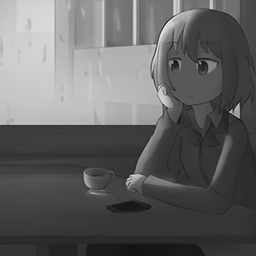
\includegraphics[width=0.4\linewidth]{images/splitbergman-after.png}
			\caption{ภาพหลังซ่อมแซมด้วยการแปรผันรวม}
		\end{subfigure}
	\end{figure}

\section{Objective}
วัตถุประสงค์ของโครงการวิจัยมีดังต่อไปนี้
\begin{description}
	\item[(1)] เพื่อลบคำบรรยายแบบ Hard ออกจากวิดีโออนิเมะ
\end{description}

\section{Scope of Study}
ขอบเขตของโครงงานมีดังต่อไปนี้
\begin{description}
\item[(3.1)] วิดีโอที่ใช้ศึกษาเป็นวิดีโอประเภทอนิเมะเท่านั้น
\item[(3.2)] บทบรรยายที่ใช้ทดสอบ จะถูกล้อมรอบไว้ด้วยสีดำ ขนาดความหนาขนาดไม่น้อยกว่า 5 พิกเซล
\item[(3.3)] จะทำการทดสอบการลบคำบรรยายบน 3 ภาษาได้แก้ ไทย จีน และอังกฤษ
\item[(3.4)] วิดีโอที่ใช้ศึกษาขนาดไม่เกิน 1920x1080
\item[(3.5)] คอมพิวเตอร์ที่ใช้ทดลองใช้หน่วยประมวลผล I7-6700HQ ใช้การ์ดจอ Nvidia GTX 960M แรม 16GB ฮาร์ดดิกส์แบบ SSD
\end{description}

\section{Methodology}
วิธีการมีดังต่อไปนี้
\begin{description}
	\item[(4.1)] พัฒนาวิธีการหาบทบรรยาย
	\item[(4.2)] ปรับปรุงความเร็วของ split begman
	\item[(4.3)] พัฒนา Avisynth Plugin สำหรับใช้กับวิดีโอ
	\item[(4.4)] เปรียบเทียบ Plug in ที่ใช้วิธีการแปรผันรวมด้วยวิธี split bergman กับวิธีอื่น
	\item[(4.5)] เขียนรายงานโครงการวิจัย
\end{description}
\section{Time Periods}
แผนการดำเนินงานตลอดทั้งโครงการสามารถสรุปได้โดยย่อจากตารางต่อไปนี้
\begin{center}
	\begin{tabular}[ht]{|l|c|c|c|c|c|c|c|c|c|c|c|c|}
		\hline
		&\multicolumn{12}{c|}{เดือนที่}\\
		\cline{2-13}
		แผนการดำเนินงาน&1&2&3&4&5&6&7&8&9&10&11&12\\
		\hline
		พัฒนาวิธีการหาบทบรรยาย&x&x& & & & & & & & & &\\
		ปรับปรุงความเร็วของ split begman& & &x&x& & & & & & & &\\
		พัฒนา Avisynth Plugin สำหรับใช้กับวิดีโอ& & & & &x&x& & & & & &\\
		เปรียบเทียบการลบซับวิธีการแปรผันรวมกับวิธีอื่น & & & & & & &x&x& & & &\\
		เขียนรายงานโครงการวิจัย& & & & & & & & &x&x&x&x\\
		\hline
	\end{tabular}
\end{center}




\section{References}

\renewcommand{\section}[2]{} % addition mod: remove reference text
\begin{thebibliography}{}
	\bibitem{ref:defination-of-inpaint} 
	Furht B., อ้างอิง 2561: Encyclopedia of Multimedia [จาก \url{https://doi.org/10.1007/0-387-30038-4_98}] สืบค้นเมื่อ 5 สิงหาคม 2561
	
	\bibitem{ref:defination-of-variation-inpaint}
	Işık Barış Fidaner, อ้างอิง 2561: A Survey on Variational Image Inpainting , Texture Synthesis and Image Completion [จาก \url{https://www.semanticscholar.org/paper/_/36f4d32ce45f72091510ab4d4d1cc3bf81ffe879}] สืบค้นเมื่อ 5 สิงหาคม 2561
	
	\bibitem{ref:splitbergman-denoise}
	Pascal Getreuer, อ้างอิง 2561:  Rudin-Osher-Fatemi Total Variation Denoising using Split Bregman , [จาก \url{https://doi.org/10.5201/ipol.2012.g-tvd}] สืบค้นเมื่อ 5 สิงหาคม 2561
	
	\bibitem{ref:splitbergman-inpaint}
	Pascal Getreuer, อ้างอิง 2561:  Total Variation Inpainting using Split Bregman , [จาก \url{https://doi.org/10.5201/ipol.2012.g-tvi}] สืบค้นเมื่อ 5 สิงหาคม 2561
	
\end{thebibliography}


\end{document}
	
	
	
	